\chapter{Valutazione dei risultati e metriche di qualità} \label{chap:evaluation}

Questo capitolo presenta le metriche comunemente utilizzate in astrofotografia, nonché quelle impiegate in questo progetto per valutare la qualità delle immagini ottenute attraverso il processo di elaborazione descritto nei capitoli precedenti.

La selezione delle metriche è fondamentale per stabilire criteri oggettivi di valutazione e per confrontare i risultati ottenuti con diverse configurazioni di parametri. Verranno discusse sia metriche con riferimento, che richiedono un'immagine ideale per il confronto, sia metriche senza riferimento, che valutano autonomamente la qualità dell'immagine

Successivamente, verranno presentati i risultati ottenuti e analizzati i miglioramenti introdotti dalle varie tecniche di elaborazione delle immagini.


\section{Metriche di valutazione con riferimento} \label{sec:r_metrics}

Le metriche con riferimento confrontano l'immagine elaborata con un'immagine ideale, fornendo una misura della similarità o della qualità relativa tra le due. Nel contesto di questo progetto, l'utilizzo di metriche con riferimento ha presentato alcune sfide, principalmente a causa dell'assenza di un'immagine di riferimento adeguata, come discusso nella \cref{sec:challenges}.

\subsection{SSIM} \label{subsec:ssim}

\textbf{SSIM} (Structural Similarity Index Measure) è una metrica che misura la similarità strutturale tra due immagini. In astrofotografia, dopo aver applicato tecniche di denoising, la metrica SSIM viene utilizzata per valutare quanto efficacemente il rumore è stato ridotto mantenendo intatte le strutture originali dell'immagine, come stelle, galassie e nebulose. SSIM può essere impiegata anche per perfezionare la tecnica dello stacking, aiutando a determinare quali combinazioni di immagini offrono la migliore preservazione delle strutture dettagliate rispetto all'immagine di riferimento.

La formula generale per il calcolo dell'SSIM tra due immagini $x$ e $y$ è:

$$
\text{SSIM}(x, y) = \frac{(2\mu_x\mu_y + C_1)(2\sigma_{xy} + C_2)}{(\mu_x^2 + \mu_y^2 + C_1)(\sigma_x^2 + \sigma_y^2 + C_2)}
$$

dove $\mu_x$ e $\mu_y$ sono le medie delle immagini $x$ e $y$, $\sigma_x^2$ e $\sigma_y^2$ sono le varianze, $\sigma_{xy}$ è la covarianza tra $x$ e $y$ e, infine, $C_1$ e $C_2$ sono due costanti che stabilizzano la divisione in caso di valori molto bassi di $\mu_x^2 + \mu_y^2$ e $\sigma_x^2 + \sigma_y^2$. Il valore dell'SSIM è compreso tra $-1$ e $1$, dove $1$ indica una similarità perfetta tra le due immagini, e $-1$ indica una dissimilarità totale.

SSIM tiene conto della percezione umana, valutando la luminanza, il contrasto e la struttura delle immagini. Tuttavia, è sensibile a piccoli spostamenti e rotazioni tra le immagini e non è in grado di valutare la qualità di immagini con diverse dimensioni o scale.

Nel progetto, a causa dell'assenza di un'immagine di riferimento adeguata (come discusso nella \cref{sec:challenges}), l'utilizzo dell'SSIM non è stato possibile.

\subsection{SNR} \label{subsec:snr}

Il \textbf{Rapporto Segnale-Rumore} (SNR: Signal-to-Noise Ratio) è una metrica fondamentale nell'ambito dell'astrofotografia, utilizzata per quantificare la qualità delle immagini astronomiche. Esso misura la relazione tra il segnale utile (le informazioni desiderate, come stelle, galassie o, in questo caso, la Luna e i suoi dettagli) e il rumore di fondo presente nell'immagine. Un alto valore di SNR indica che il segnale è dominante rispetto al rumore, risultando in immagini più nitide e dettagliate. 

Generalmente l'SNR si calcola a partire dalla normalizzazione dell'errore quadratico medio o di altre metriche di errore relative, come segue:

$$
SNR = 10 \cdot \log_{10} (\xi)
$$

$\xi$ è l'errore relativo calcolato scondo formule come:

\begin{enumerate}
    \item Normalized Least Squares Error (NLSE):
    $$
    \xi_{NLSE} = \dfrac{\sum_{j = 1}^J \sum_{k=1}^K |F(j, k) - \hat F(j, k)|^2}
    {\sum_{j = 1}^J \sum_{k=1}^K |F(j, k)|^2}
    $$

    \item Peak Least Squares Error (PLSE):
    $$
    \xi_{PLSE} = \dfrac{\sum_{j = 1}^J \sum_{k=1}^K |F(j, k) - \hat F(j, k)|^2}
    {[\text{MAX}\{F(j, k)\}]^2}
    $$
\end{enumerate}

dove $F(j, k)$ è il valore del pixel originale, $\hat F(j, k)$ è il valore del pixel elaborato, $J$ e $K$ sono le dimensioni dell'immagine e $\text{MAX}\{F(j, k)\}$ è il valore massimo del pixel nell'immagine originale.

Una formula semplificata e comunemente utilizzata per calcolare l'SNR è:

$$
SNR = 10\cdot \log_{10} \left(\dfrac{\mu_s^2}{\sigma_n^2}\right)
$$

dove $\mu_s$ è la media del segnale e $\sigma_n$ è la deviazione standard del rumore.

L'SNR è una metrica semplice e intuitiva, ma non tiene conto delle caratteristiche percettive del sistema visivo umano. Inoltre, come SSIM, è sensibile a piccoli spostamenti e rotazioni tra le immagini e non è in grado di valutare la qualità di immagini con diverse dimensioni o scale, richiedendo dunque un perfetto allineamento tra le immagini di riferimento e quelle elaborate.

Algoritmi di denoising avanzati, inclusi quelli basati su reti neurali, vengono valutati utilizzando l'SNR per garantire che il segnale sia preservato efficacemente mentre il rumore viene minimizzato. Tuttavia, anche l'SNR non è stato utilizzato in questo progetto a causa dell'assenza di un'immagine di riferimento adeguata.

\section{Metriche di valutazione senza riferimento} \label{sec:nr_metrics}

La mancanza di un'immagine di riferimento ideale ha reso necessario l'utilizzo di metriche di valutazione senza riferimento per valutare la qualità delle immagini elaborate.

Le metriche senza riferimento valutano la qualità dell'immagine in maniera autonoma, senza bisogno di confrontarla con un'immagine ideale,analizzando dunque l'immagine stessa per stimare la sua qualità basandosi su modelli statistici o percettivi.

\subsection{NIQE} \label{subsec:niqe}

\textbf{NIQE} (Naturalness Image Quality Evaluator) è una metrica di qualità delle immagini senza riferimento, sviluppata per valutare autonomamente la qualità delle immagini digitali, senza necessità di un'immagine di riferimento. NIQE è basata su un modello di percezione visiva umana, che valuta la qualità dell'immagine basandosi su caratteristiche statistiche e percettive, come la nitidezza, il contrasto, la luminosità e la presenza di artefatti \cite{niqe}.

NIQE calcola la distanza tra le statistiche dell'immagine e quelle di un campione di immagini di riferimento, fornendo un punteggio di qualità (generalmente tra 0 e 100) che indica quanto l'immagine si discosti dalla media delle immagini di riferimento. Punteggi più bassi indicano una qualità migliore.

Nel progetto, NIQE è stata testata come possibile metrica di valutazione, ma ha mostrato limitazioni nel catturare miglioramenti specifici apportati dalle tecniche di elaborazione applicate alle immagini lunari. Ciò è probabilmente dovuto alla natura specifica delle immagini lunari, che possono differire significativamente dalle immagini di riferimento utilizzate per addestrare il modello.

\subsection{BRISQUE} \label{subsec:brisque}

\textbf{BRISQUE} (Blind Referenceless Image Spatial Quality Evaluator) è una metrica di qualità delle immagini senza riferimento che valuta le distorsioni naturali basandosi su modelli statistici delle scene naturali \cite{brisque}. A differenza di NIQE, BRISQUE utilizza un approccio di apprendimento supervisionato, addestrato su un ampio dataset di immagini con varie distorsioni.

BRISQUE estrae caratteristiche statistiche dall'immagine, come la distribuzione dei coefficienti MSCN (Mean Subtracted Contrast Normalized), per catturare le deviazioni dalla naturalità statistica tipicamente presenti nelle immagini di alta qualità. Il modello produce un punteggio in una scala da 0 a 100, dove punteggi più bassi indicano qualità migliore.

Nel contesto del progetto, BRISQUE ha dimostrato una maggiore sensibilità rispetto a NIQE nel rilevare miglioramenti nella qualità dell'immagine, ma ha presentato alcune limitazioni nell'analisi di immagini astronomiche, che differiscono significativamente dalle scene naturali su cui il modello è stato addestrato.

\subsection{LIQE} \label{subsec:liqe}

\textbf{LIQE} (Learning-based Image Qu  ality Evaluator) è una metrica di qualità delle immagini senza riferimento basata su tecniche di \textit{deep learning} avanzate \cite{liqe}. Si distingue per la sua capacità di combinare efficacemente informazioni statistiche a livello sia globale che locale, permettendo una valutazione più accurata delle distorsioni presenti nelle immagini.

Il modello assegna un punteggio in una scala da 1 a 5, dove 1 indica una qualità molto bassa e 5 una qualità molto alta. Si noti che questa scala è adottata nell'implementazione della libreria \texttt{PyIQA}, altre implementazioni potrebbero utilizzare scale diverse (generalmente 0-100).

La caratteristica distintiva di LIQE rispetto a NIQE e BRISQUE è la sua architettura basata su reti neurali convoluzionali profonde, addestrate su un vasto dataset di immagini con varie distorsioni. Questo approccio rende LIQE particolarmente robusto e versatile nella valutazione di diverse tipologie di immagini.

\subsection{Considerazioni sulle metriche} \label{subsec:why_liqe}

Nel progetto, sono state implementate e testate diverse metriche di valutazione senza riferimento, tra cui NIQE, BRISQUE e LIQE, utilizzando la libreria \texttt{PyIQA}, che fornisce implementazioni pronte all'uso di diverse metriche di qualità delle immagini.

Dopo aver valutato i risultati ottenuti, è emerso che \textbf{LIQE risulta la metrica più adatta} per valutare la qualità delle immagini lunari elaborate. Questa scelta è stata motivata da diversi fattori: innanzitutto, a causa dell'assenza di un'immagine di riferimento ideale, le metriche con riferimento non erano applicabili nel contesto del progetto; tra le metriche senza riferimento, LIQE ha dimostrato di essere più sensibile ai miglioramenti apportati dalle tecniche di elaborazione implementate.

Durante lo sviluppo, è emerso che metriche come NIQE e BRISQUE non sempre riflettevano accuratamente la percezione umana della qualità delle immagini. Ad esempio, in alcuni casi, un'immagine che visivamente appariva migliorata presentava un punteggio peggiore secondo queste metriche. LIQE, invece, ha mostrato una maggiore correlazione con la qualità percepita.

È importante notare che LIQE non è progettato per valutare immagini astronomiche. Il modello (normalizzato tra 1 e 5), assegna valori che si aggirano intorno a 2, indicando una qualità molto bassa. Probabilmente ciò è dovuto al fatto che il modello è stato addestrato su un dataset di immagini a colori, mentre la Luna è pressocché monocromatica. Tuttavia si può notare che a miglioramenti visivi delle immagini corrispondevano incrementi nei punteggi LIQE, e viceversa.

\section{Analisi e miglioramenti ottenuti} \label{sec:analysis}

In questa sezione vengono analizzati i risultati ottenuti attraverso l'applicazione delle diverse tecniche di elaborazione descritte nei capitoli precedenti. L'obiettivo è valutare l'efficacia di ciascuna fase del processo nel migliorare la qualità delle immagini lunari, utilizzando le metriche di valutazione senza riferimento discusse nel \cref{chap:evaluation}. Verranno presentati grafici, tabelle e immagini illustrative per supportare l'analisi e facilitare il confronto tra i vari metodi.

Nell'analisi dei grafici si ricorda che le metriche NIQE e BRISQUE assegnano punteggi su una scala da 0 a 10, im modo che valori più bassi corrispondano a immagini di qualità migliore. LIQE, al contrario, assegna punteggi in una scala da 1 a 5, dove valori più alti corrispondono a immagini di qualità superiore.

\subsection{Effetti della calibrazione} \label{subsec:analysis_cal}

La calibrazione delle immagini è un passaggio fondamentale nell'astrofotografia per rimuovere artefatti strumentali e migliorare il rapporto segnale-rumore. In questa sezione si analizza l'impatto della calibrazione sulle immagini lunari acquisite, confrontando le metriche di qualità prima e dopo l'applicazione della calibrazione.

\begin{figure}[H]
    \centering
    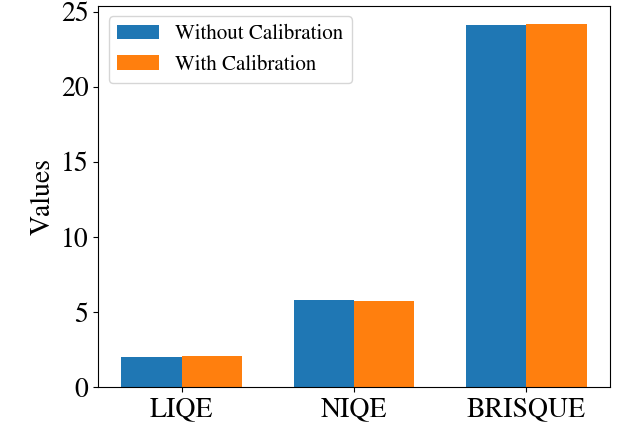
\includegraphics[scale = 0.475]{../assets/calibration_effect.png}
    \caption{Confronto tra le metriche sull'immagine finale con e senza calibrazione.}
    \label{fig:confronto-calibrazione}
\end{figure}

Dai dati raccolti, si osserva che la calibrazione non ha comportato un miglioramento significativo nelle metriche di qualità. Ricordando che nell'ambito di questo progetto si è deciso di non usare i bias frames, in quanto difficili da ottenere, si può ipotizzare che l'assenza di una calibrazione più completa abbia limitato i miglioramenti ottenibili. In ogni caso, la lieve differenza tra i risultati con immagini calibrate e non suggerisce due alternative:
\begin{enumerate}
    \item le immagini originali erano già ben bilanciate e prive di distorsioni significative.
    \item le fasi successive di elaborazione hanno compensato eventuali difetti presenti nelle immagini non calibrate.
\end{enumerate}

Questa fase assume particolare importanza quando si lavora con immagini astronomiche dello spazio profondo, dove la luminosità dei soggetti è molto bassa e la presenza di artefatti strumentali è più evidente. Nel caso di immagini lunari, la calibrazione potrebbe non essere necessaria se le immagini sono già di alta qualità.

\subsection{Impatto del denoising} \label{subsec:analysis_den}

Il denoising è essenziale per attenuare il rumore presente nelle immagini senza degradare i dettagli importanti. Sono stati testati diversi metodi di denoising, tra cui DnCNN, filtro gaussiano, filtro bilaterale e filtro mediano.

Analizziamo innanzi tutto come si presentano visivamente le immagini elaborate con i diversi metodi di denoising:

\begin{figure}[H]
    \centering
    \begin{tikzpicture}
        % Immagine centrale (originale)
        \node[anchor=center] (original) at (0, 0) {
            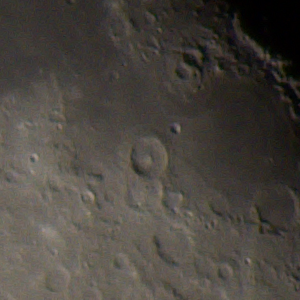
\includegraphics[width=0.25\textwidth]{../assets/original_zoom.png}
        };
        \node[below=0cm of original] {(e) Originale};
        
        % Immagine in alto a sinistra
        \node[anchor=center] (top-left) at (-4, 2.25) {
            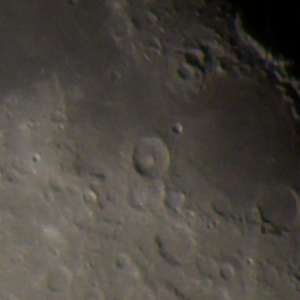
\includegraphics[width=0.25\textwidth]{../assets/den_median_zoom.png}
        };
        \node[below=0cm of top-left] {(a) Filtro mediano}; 
        
        % Immagine in alto a destra
        \node[anchor=center] (top-right) at (4, 2.25) {
            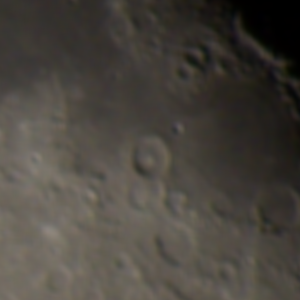
\includegraphics[width=0.25\textwidth]{../assets/den_gaussian_zoom.png}
        };
        \node[below=0cm of top-right] {(b) Filtro gaussiano}; 
        
        % Immagine in basso a sinistra
        \node[anchor=center] (bottom-left) at (-4, -2.25) {
            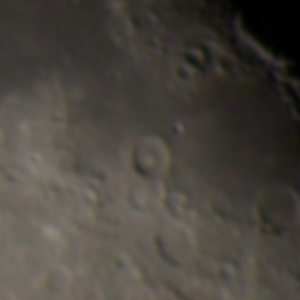
\includegraphics[width=0.25\textwidth]{../assets/den_bilateral_zoom.png}
        };
        \node[below=0cm of bottom-left] {(c) Filtro bilaterale}; 
        
        % Immagine in basso a destra
        \node[anchor=center] (bottom-right) at (4, -2.25) {
            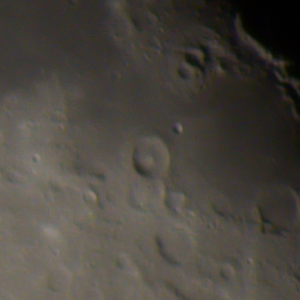
\includegraphics[width=0.25\textwidth]{../assets/den_dncnn_zoom.png}
        };
        \node[below=0cm of bottom-right] {(d) DnCNN}; 
    \end{tikzpicture}
    \caption{Confronto tra diversi filtri di riduzione del rumore.}
    \label{fig:confronto-filtri}
\end{figure}

la \cref{fig:confronto-filtri} mostra un confronto tra le immagini ottenute applicando i diversi filtri ad un'immagine del set iniziale, ingrandite di un fattore 5 su una zona che presenta crateri, pianure e penombra, in modo da evidenziare il comportamento dei filtri nelle diverse situazioni. Da un'attenta analisi visiva si può notare che, rispetto all'originale:

\begin{itemize}
    \item Il filtro gaussiano introduce una sfocatura diffusa che riduce il rumore in maniera significativa, ma penalizza fortemente la nitidezza. I dettagli più fini, come i bordi dei crateri, risultano appiattiti e meno definiti, rendendo l'immagine visivamente "morbida" e poco adatta per analisi dettagliate.

    \item Il filtro mediano riduce il rumore in maniera aggressiva, eliminando molte irregolarità. Tuttavia, questa operazione comporta una perdita di dettagli nei contorni e nei bordi, che appaiono meno definiti. I crateri lunari perdono profondità e risultano leggermente appiattiti.

    \item Il filtro bilaterale offre un buon compromesso tra riduzione del rumore e mantenimento dei dettagli. Sebbene non elimini completamente il rumore, i contorni rimangono relativamente definiti e i crateri conservano una certa profondità e definizione.

    \item DnCNN (Deep Learning) riduce il rumore in modo efficace mantenendo una buona nitidezza complessiva. Tuttavia, può introdurre una texture artificiale che risulta meno naturale rispetto agli altri filtri. Le strutture principali rimangono ben visibili, ma alcune sfumature possono sembrare meno realistiche.
\end{itemize}

La caratteristica innaturale di DnCNN svanisce poi con l'applicazione dell'algoritmo di unsarp masking personalizzato, che, integrando il risultato con l'immagine di partenza, permette di mantenere la nitidezza e la naturalezza dell'immagine.

La \cref{fig:confronto-denoising} mostra i risultati ottenuti utilizzando ciascun metodo all'interno della funzione \texttt{custom\_unsharp\_mask} illustrata nella \cref{subsec:preprocessing_impl}. I punteggi delle metriche di qualità NIQE, BRISQUE e LIQE sono stati calcolati per ciascuna immagine dopo l'applicazione dell'intera pipeline di elaborazione.

\begin{figure}[H]
    \centering
    \begin{subfigure}[t]{0.32\textwidth}
        \centering
        \caption{NIQE}
        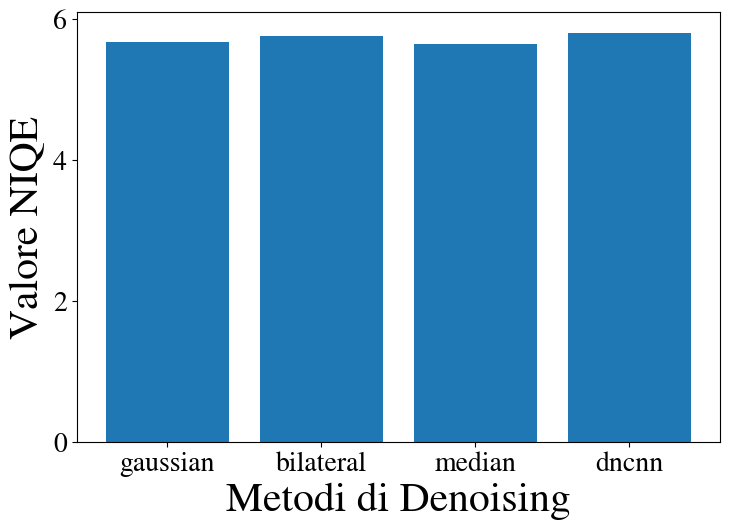
\includegraphics[width=\linewidth]{../assets/denoising_comparison_NIQE.png}
        \label{fig:den_niqe}
    \end{subfigure}
    \hfill
    \begin{subfigure}[t]{0.32\textwidth}
        \centering
        \caption{BRISQUE}
        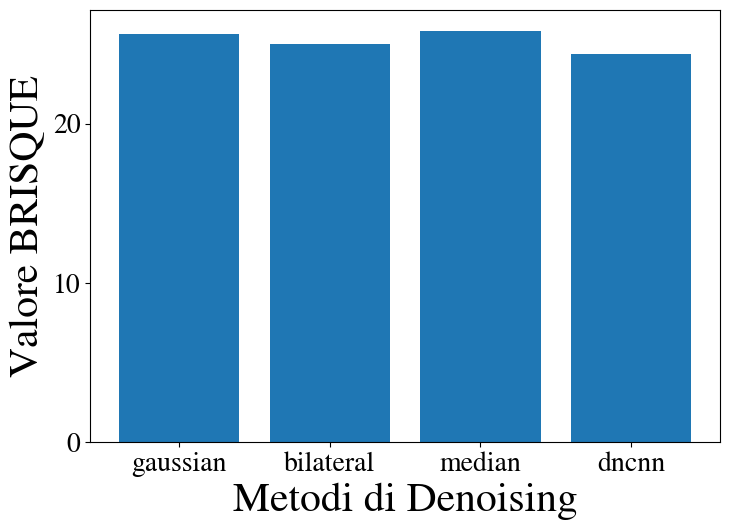
\includegraphics[width=\linewidth]{../assets/denoising_comparison_BRISQUE.png}
        \label{fig:den_brisque}
    \end{subfigure}
    \hfill
    \begin{subfigure}[t]{0.32\textwidth}
        \centering
        \caption{LIQE}
        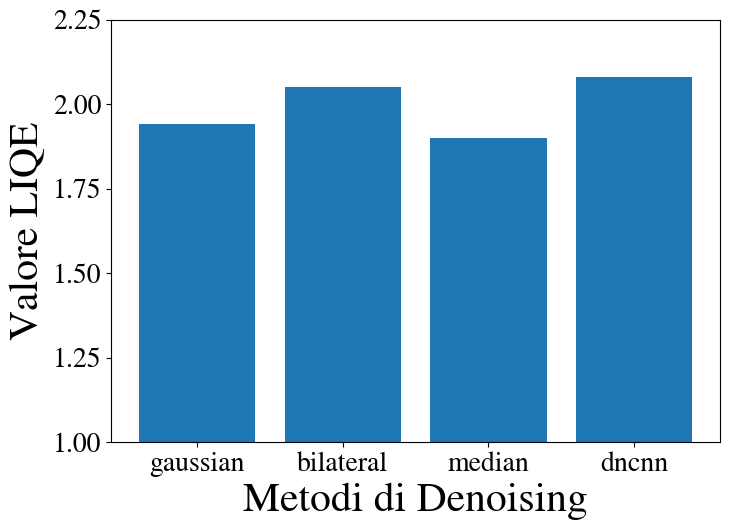
\includegraphics[width=\linewidth]{../assets/denoising_comparison_LIQE.png}
        \label{fig:den_liqe}
    \end{subfigure}
    \caption{Punteggi delle metriche di qualità sulle immagini elaborate, utilizzando i diversi metodi di denoising nella funzione \texttt{custom\_unsharp\_mask}.} \label{fig:confronto-denoising}
\end{figure}

Dai risultati ottenuti, possiamo notare che secondo la metrica NIQE i diversi metodi di denoising hanno prodotto risultati simili, con punteggi medi intorno a 5. Tuttavia, BRISQUE e LIQE hanno mostrato differenze più significative tra i metodi. In particolare, LIQE ha evidenziato una maggiore sensibilità ai dettagli, con punteggi più alti per il metodo DnCNN rispetto agli altri metodi.

È interessante notare come alcuni metodi tradizionali come il filtro bilaterale hanno mostrato performance comparabili in determinate situazioni.

\subsection{Benefici dello stacking} \label{subsec:analysis_stack}

Ormai è notoche lo stacking delle immagini consente di migliorare il rapporto segnale-rumore combinando più scatti dello stesso soggetto. Nell'ambito di questo progetto sono stati testati diversi i metodi di stacking presentati nella \cref{subsec:stacking} e implementati nella \cref{subsec:stacking_impl}, di seguito confrontati attraverso le metriche di qualità NIQE, BRISQUE e LIQE.

\begin{figure}[H]
    \centering
    \begin{subfigure}[t]{0.49\textwidth}
        \centering
        \caption{NIQE}
        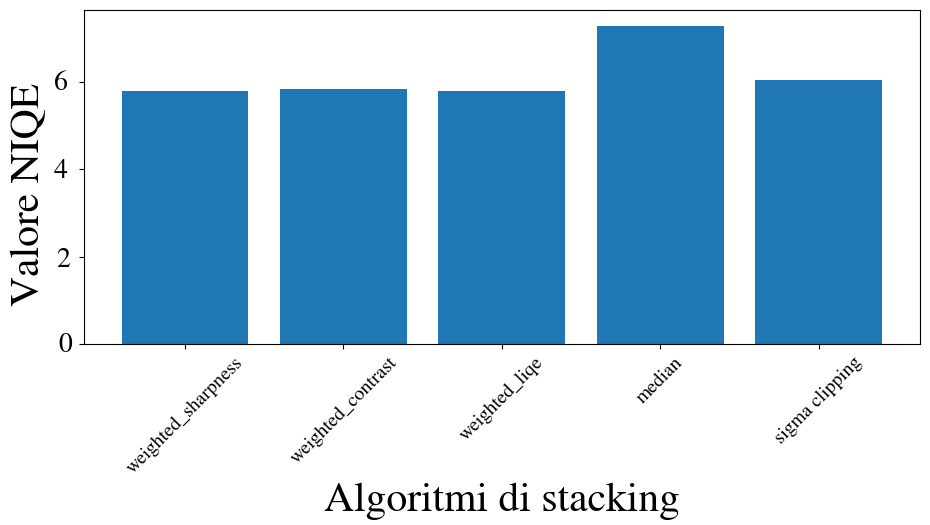
\includegraphics[width=\linewidth]{../assets/stack_NIQE.png}
        \label{fig:stack_niqe}
    \end{subfigure}
    \hfill
    \begin{subfigure}[t]{0.49\textwidth}
        \centering
        \caption{BRISQUE}
        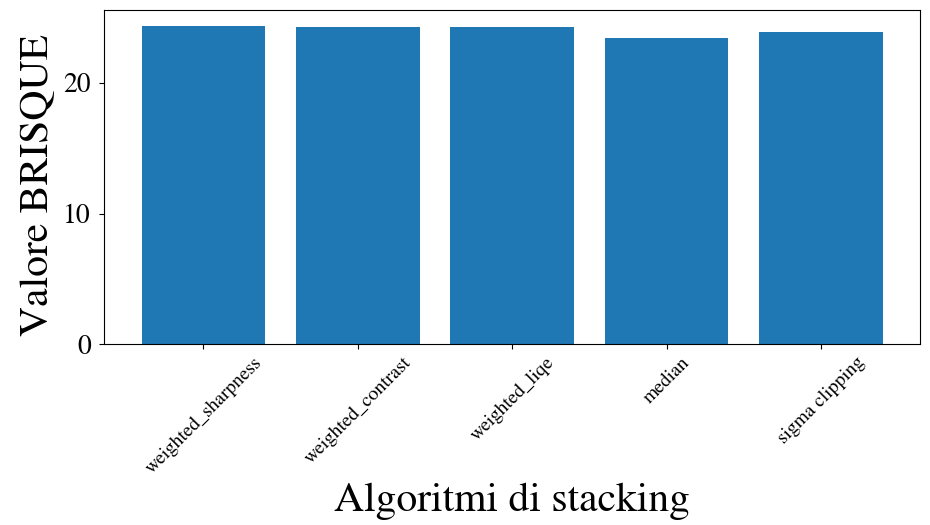
\includegraphics[width=\linewidth]{../assets/stack_BRISQUE.png}
        \label{fig:stack_brisque}
    \end{subfigure}
    \hfill
    \begin{subfigure}[t]{0.49\textwidth}
        \centering
        \caption{LIQE}
        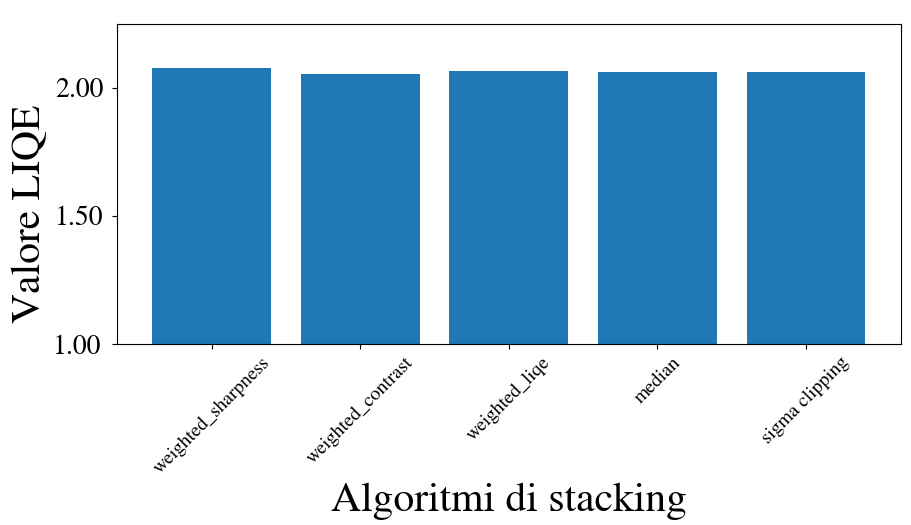
\includegraphics[width=\linewidth]{../assets/stack_LIQE.png}
        \label{fig:stack_liqe}
    \end{subfigure}
    \caption{Confronto tra diversi metodi di stacking.}
    \label{fig:confronto-stacking}
\end{figure}

Da questi risultati si evinche che la metrica BRISQUE non ha mostrato differenze significative tra i diversi metodi di stacking, con punteggi medi intorno a 24. NIQE ha mostrato una maggiore variabilità tra i metodi, con punteggi più alti (peggiori) per lo stacking mediano e inferiori (migliori) per il metodo con la media pesata, indipendentemente dai criteri di assegnazione dei pesi. Anche LIQE, come BRISQUE, ha mostrato punteggi simili tra i diversi metodi di stacking, con valori che si aggirano intorno a 2.06 per i vari metodi, tranne per la media pesata mediante nitidezza che ha un punteggio di poco superiore agli altri: 2.08.

Si vuole far notare che LIQE agisce su una scala nettamente diversa dalle altre due metriche, per cui punteggi con variabilità minore possono nascondere differenze più significative.

Per un'analisi più completa è stato analizzato l'andamento delle metriche all'aumentare del numero di immagini utilizzate nello stacking.

\begin{figure}[H]
    \centering
    \begin{subfigure}[t]{0.325\textwidth}
        \centering
        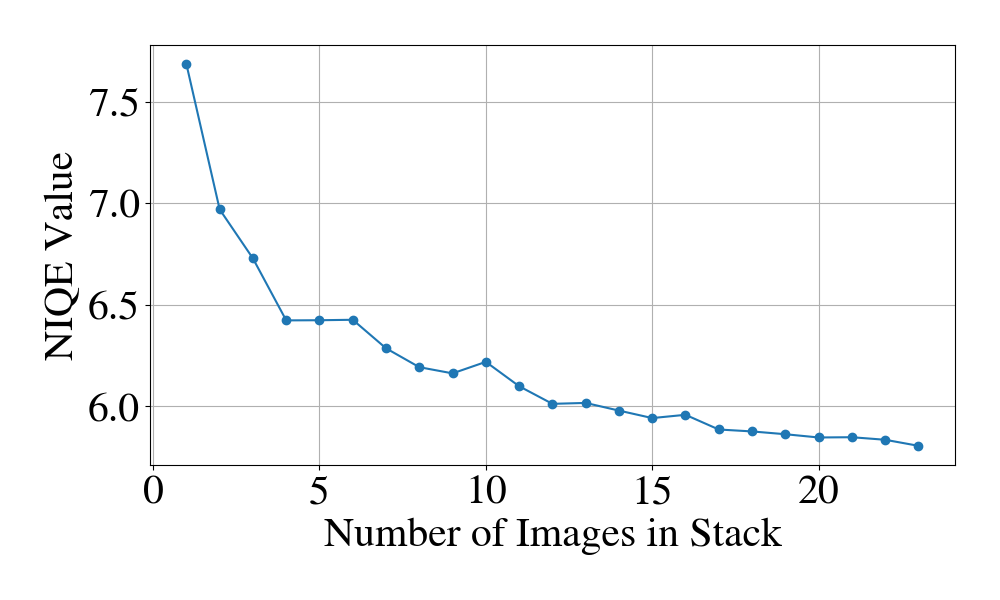
\includegraphics[width=\linewidth]{../assets/n_stack_NIQE.png}
        \caption{NIQE}
        \label{fig:n_stack_niqe}
    \end{subfigure}
    \hfill
    \begin{subfigure}[t]{0.325\textwidth}
        \centering
        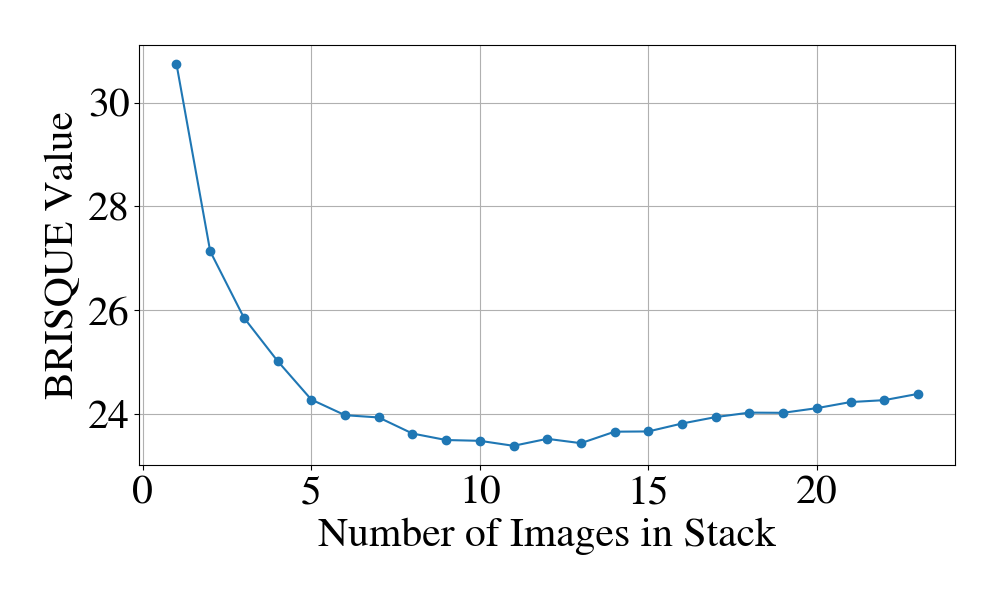
\includegraphics[width=\linewidth]{../assets/n_stack_BRISQUE.png}
        \caption{BRISQUE}
        \label{fig:n_stack_brisque}
    \end{subfigure}
    \hfill
    \begin{subfigure}[t]{0.325\textwidth}
        \centering
        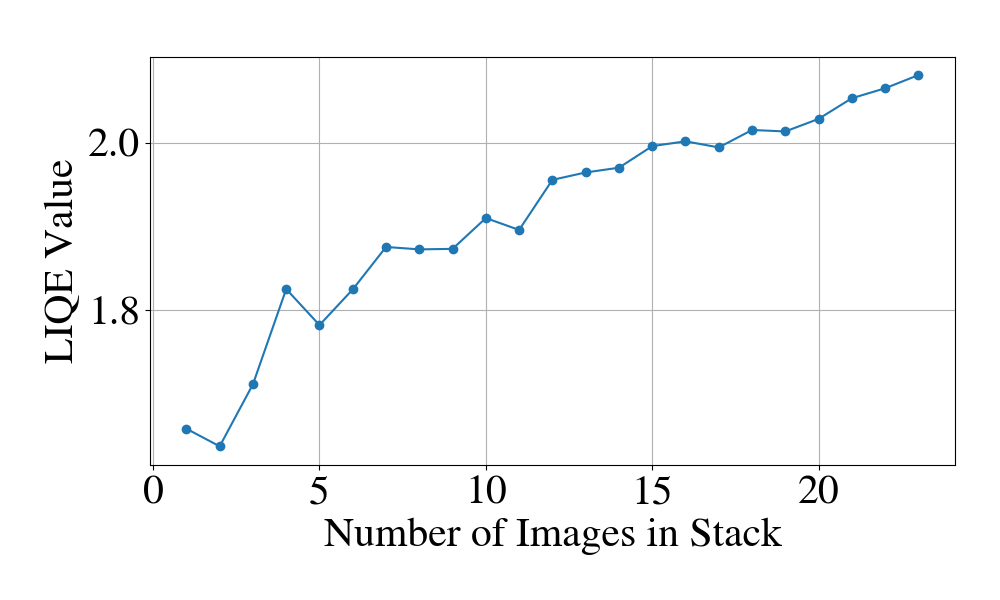
\includegraphics[width=\linewidth]{../assets/n_stack_LIQE.png}
        \caption{LIQE}
        \label{fig:n_stack_liqe}
    \end{subfigure}
    \caption{Impatto del numero di immagini in stacking sulla qualità finale.}

\end{figure}

I risultati evidenziano che l'incremento del numero di immagini porta a un netto miglioramento nelle metriche di qualità, confermando l'efficacia di questa tecnica. Di seguito sono riportate le immagini ottenute con lo stacking di 5, 10 e 20 immagini.

\begin{figure}[H]
    \centering
    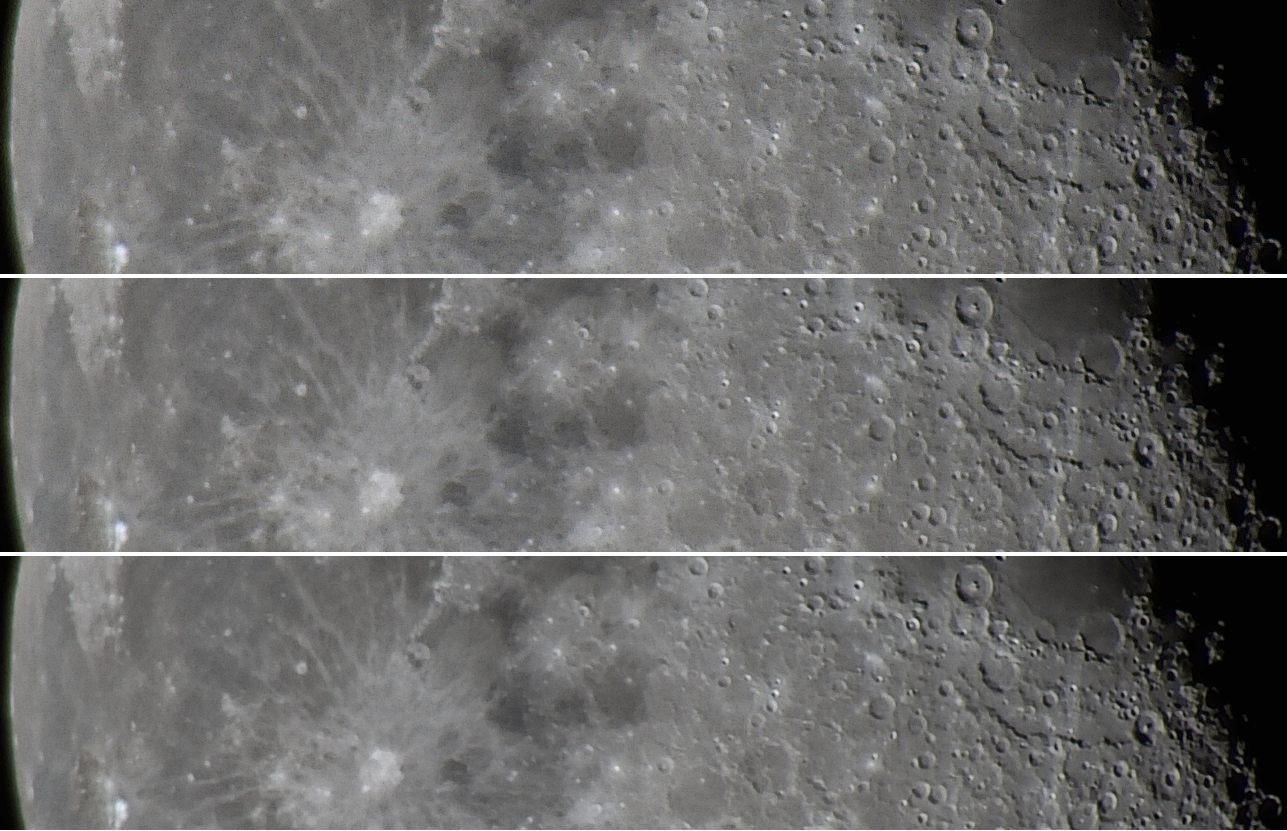
\includegraphics[width = \linewidth]{../assets/n_stack_img.png}
    \caption{Immagini ottenute con stacking di 5, 10 e 20 immagini.}
    \label{fig:n_stack_img}
\end{figure}

\subsection{Miglioramenti con sharpening e contrasto} \label{subsec:analysis_post}

L'applicazione di tecniche di post-processing, come l'aumento della nitidezza tramite Unsharp Mask e il miglioramento del contrasto con CLAHE, sono quelle che in termini di qualità percepita apportano i miglioramenti più evidenti. In questa sezione si analizzano gli effetti di queste tecniche sulle immagini lunari elaborate.

% [Inserire immagini che mostrano le differenze prima e dopo l'applicazione delle tecniche di post-processing]

Dall'analisi emerge che l'applicazione dell'Unsharp Mask ha permesso di enfatizzare i dettagli superficiali della Luna, migliorando la nitidezza percepita. Il miglioramento del contrasto con CLAHE ha reso più visibili le variazioni tonali, contribuendo a una maggiore profondità dell'immagine.

Le metriche di qualità riflettono questi miglioramenti, con punteggi più elevati nelle immagini post-processate.

\subsection{Analisi complessiva e discussione finale}

Combinando i risultati delle diverse fasi di elaborazione, si può valutare l'efficacia complessiva del processo sviluppato. Le immagini finali ottenute presentano un significativo miglioramento rispetto agli scatti originali, sia in termini di qualità percepita che secondo le metriche utilizzate.

\begin{figure}[H]
    \centering
    \caption{valore di LIQE con l'avanzare della pipeline di elaborazione}
    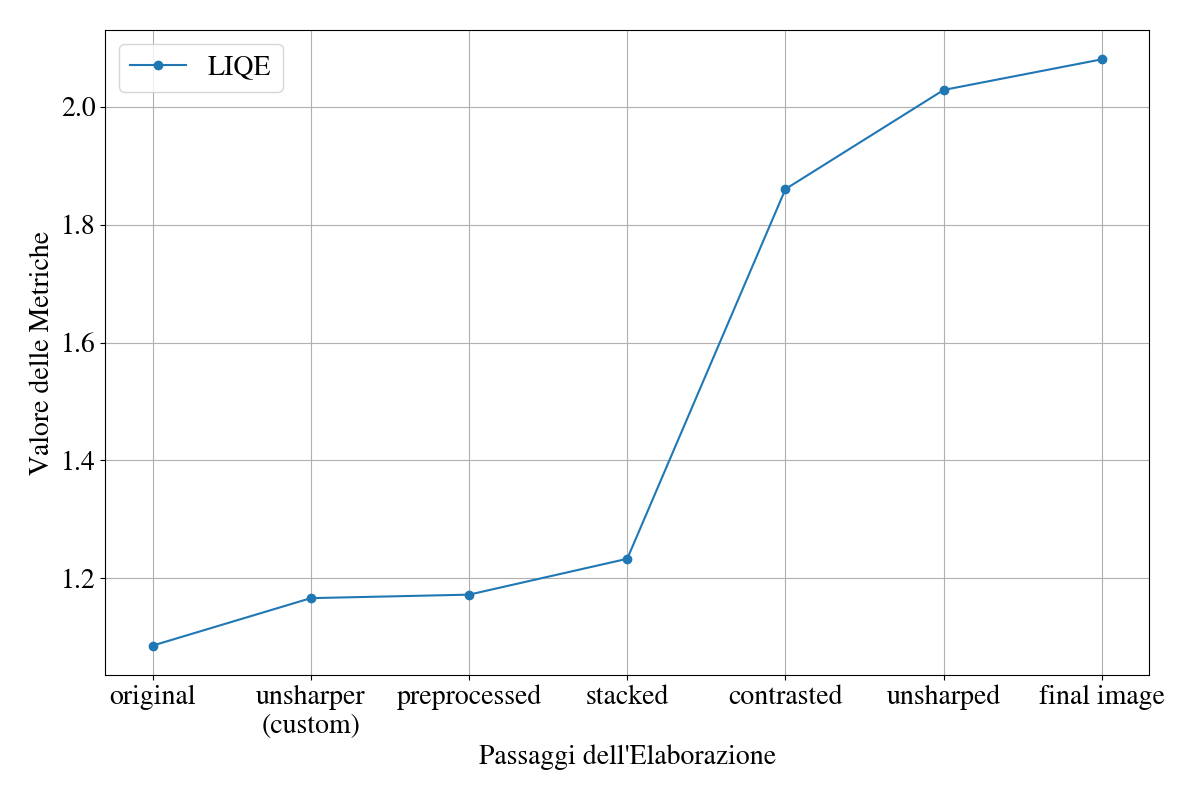
\includegraphics[width=\linewidth]{../assets/overall.png}
    \label{fig:overall}
\end{figure}

Dai risultati ottenuti, emerge che l'applicazione combinata delle tecniche di custom unsharp mask, stacking, aumento del contrasto e sharpening ha portato a un netto miglioramento nella qualità delle immagini lunari. 

È interessante notare che la tecniche che hanno mostrato il maggior impatto sulla qualità finale sono quelle di postprocessing, come l'aumento della nitidezza e del contrasto. A primo impatto potrebbe sembrare che fasi come il custom unsharp masking, o lo stacking abbiano un impatto minore sul risultato finale, ma è importante sottolineare che senza queste fasi, le tecniche di postprocessing non avrebbero potuto ottenere risultati altrettanto significativi (\cref{fig:overall_no}).

\begin{figure}[H]
    \begin{subfigure}[t]{0.49\textwidth}
        \centering
        \caption{Pipeline senza custom unsharp mask}
        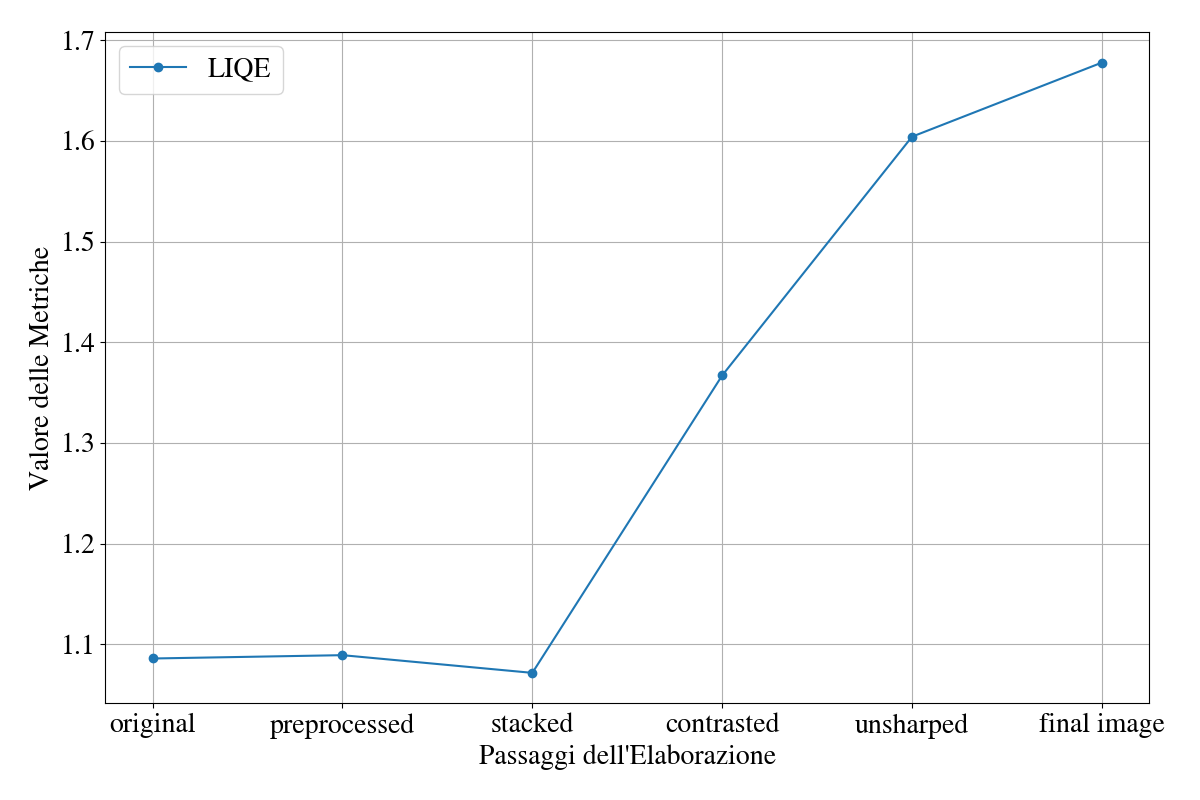
\includegraphics[width=\linewidth]{../assets/overall_no_ush.png}
        \label{fig:overall_no_ush}
    \end{subfigure}
    \hfill
    \begin{subfigure}[t]{0.49\textwidth}
        \centering
        \caption{Pipeline senza stacking}
        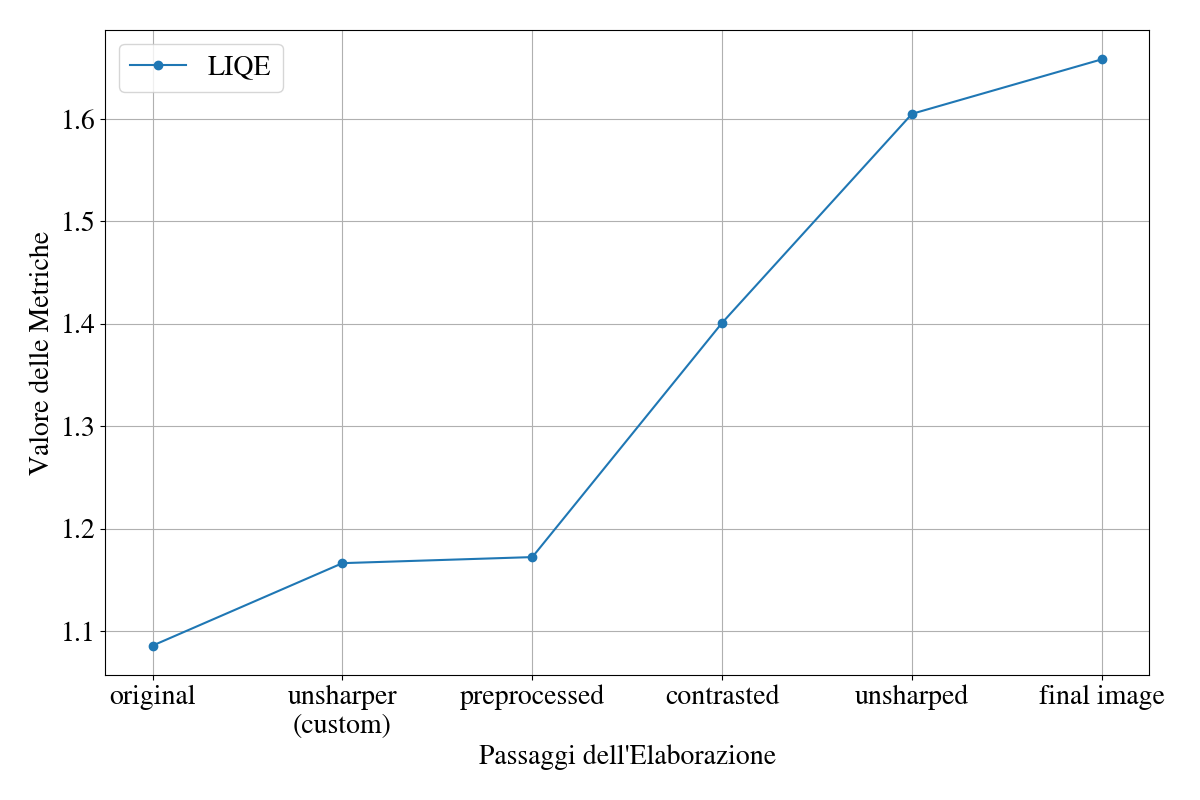
\includegraphics[width=\linewidth]{../assets/overall_no_stack.png}
        \label{fig:overall_no_stack}
    \end{subfigure}
    \caption{Impatto delle fasi di custom unsharp mask e stacking sulla qualità finale.}
    \label{fig:overall_no}
\end{figure}

\cleardoublepage